\documentclass[a4paper]{article}
\usepackage[utf8x]{inputenc}
\usepackage[russian]{babel}
\usepackage[dvips]{graphicx}
%\usepackage{mathtext}
\usepackage{indentfirst}  % абзацный отступ после заголовка
\usepackage{misccorr}  % точка в заголовке
%\frenchspacing  % без пробелов после предложений
\usepackage{longtable}
\usepackage{verbatim}
\usepackage{setspace}

\addtolength{\hoffset}{-2.4cm}
\addtolength{\textwidth}{4.8cm} 
\parindent=15mm
\onehalfspacing % полутроный интервал

% установка номера страницы на верхнем колонтитуле
\usepackage{fancyhdr} % пакет для установки колонтитулов
\pagestyle{fancy} % смена стиля оформления страниц
\fancyhf{} % очистка текущих значений
\fancyhead[C]{\thepage} % установка верхнего колонтитула
\renewcommand{\headrulewidth}{0pt} % убрать разделительную линию 

\begin{document}
\begin{titlepage}
\begin{center}

\fontsize{14pt}{18pt}
\selectfont

\vfill
Федеральное агентство по образованию РФ\\
Новгородский государственный университет им.~Ярослава~Мудрого

\hrulefill

Кафедра ИТИС

\vfill
\vfill

{
\huge
Реализация алгоритмов поиска корней~уравнений\linebreak
методом половинного деления и методом хорд
}

\vfill

{
\begin{flushright}
Выполнил студент группы 9311\\
Лопатин А.С.
\end{flushright}
}

\vfill

Великий Новгород, 2009
\end{center}
\end{titlepage}

\fontsize{14pt}{18pt}
\selectfont

\section{Цель работы}
Цель работы --- реализовать алгоритм поиска корней уравнения
методом половинного деления и методом хорд на языке программирования Pascal.

\section{Математическая модель решения}
Даны границы $a$, $b$ и точность $\varepsilon$.
Необходимо найти корень уравнения
(например квадратичного~$y=10x-2x^2$ или линейного~$y=2x-20$ уравнения)
между границами, который соответствует заданной точности,
т.~е. значение переменной $x$ при
$|y| \le \varepsilon$ или при $|b-a|\le\varepsilon$.

Проверить наличие корней уравнения можно по формуле $F(a)\times F(b)$.
Если значение отрицательное --- корни есть.

Вычислять же корень можно с помощью разделения суммы границ пополам
($x=\frac{a+b}{2}$) или выразив $x$ из
уравнения прямой ($x=\frac{F(b)\times a-F(a) \times b}{F(b)-F(a)}$).
После этого надо установить значение новой границы $a$ или $b$
равным найденному $x$ в зависимости от $F(a)\times F(x)$
(для отрицательных --- $b$, для остальных --- $a$)
и проверить результат на соответствие точности $\varepsilon$
(определяется либо по формуле $|F(x)|\le\varepsilon$
либо через $|b-a|\le\varepsilon$).
Также, для метода хорд был найден оптимальный способ проверить точность
с помощью $y$, выраженного из уравнения прямой:
$|\frac{F(b)\times a-F(a) \times b}{F(b)-F(a)}-x|\le\varepsilon$.

\section{Спецификация}
Таблица переменных:

{
\fontsize{10pt}{12pt}
\selectfont
\parindent=0mm
\begin{longtable}{|p{1.5cm}|l|l|l|c|p{4cm}|}
\hline
Исходное значение & Идентификатор & Тип & Вид & Размерность & Назначение\\
\hline
$a$ & a & Вещественный & Простой & -- & Левая граница\\
\hline
$b$ & b & Вещественный & Простой & -- & Правая граница\\
\hline
$\varepsilon$ & eps & Вещественный & Простой & -- & Точность\\
\hline
$x$ & x & Вещественный & Простой & -- & Корень уравнения\\
\hline
$y$ & y & Вещественный & Простой & -- & Значение функции $F(x)$\\
\hline
$y_1$ & y1 & Вещественный & Простой & -- & Значение функции $F(a)$\\
\hline
$y_2$ & y2 & Вещественный & Простой & -- & Значение функции $F(b)$\\
\hline
$i$ & i & Целый & Простой & -- & Номер итерации\\
\hline
function number & func\_number & Целый & Простой & -- & Номер функции\\
\hline
calculation method & calc\_method & Целый & Простой & -- & Метод решения\\
\hline
exactness type & excat\_type & Целый & Простой & -- & Тип точности\\
\hline
\end{longtable}
}

\section{Алгоритм}
\subsection{Главный модуль}
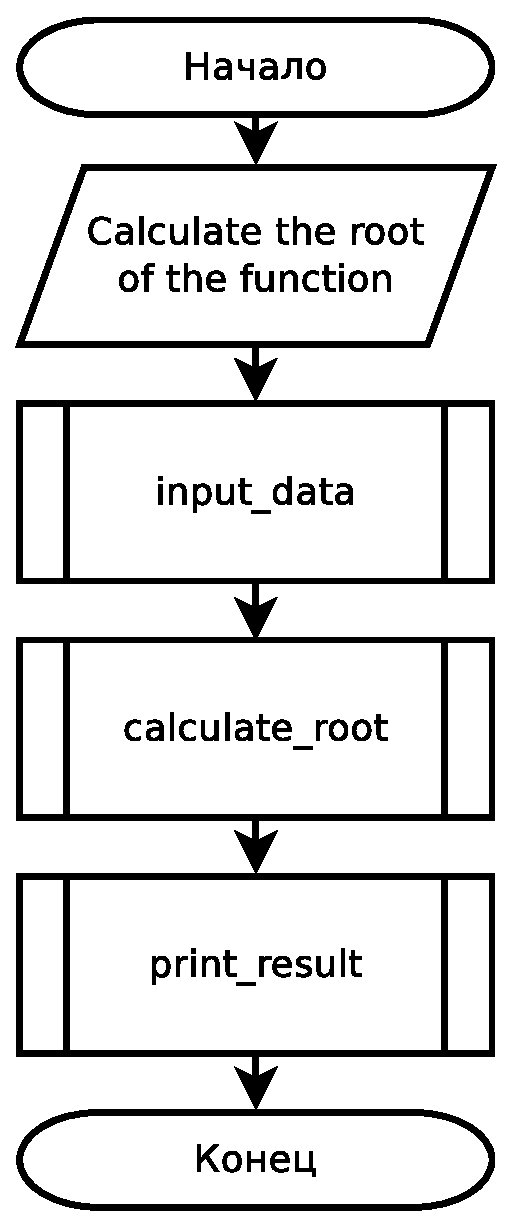
\includegraphics[scale=0.5]{schemes/main}

\subsection{Процедура <<input\_data>>}
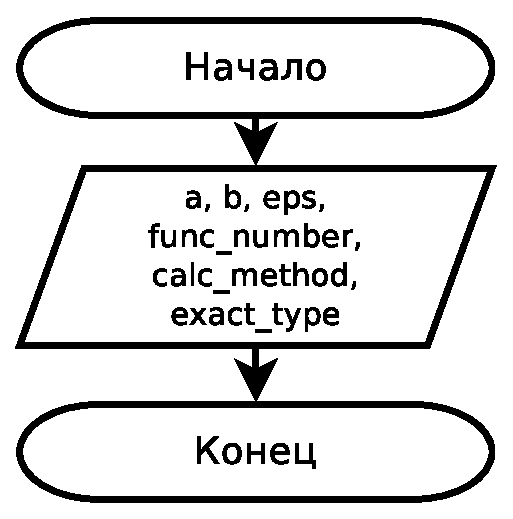
\includegraphics[scale=0.5]{schemes/input_data}

\subsection{Функция <<$F(x)$>>}
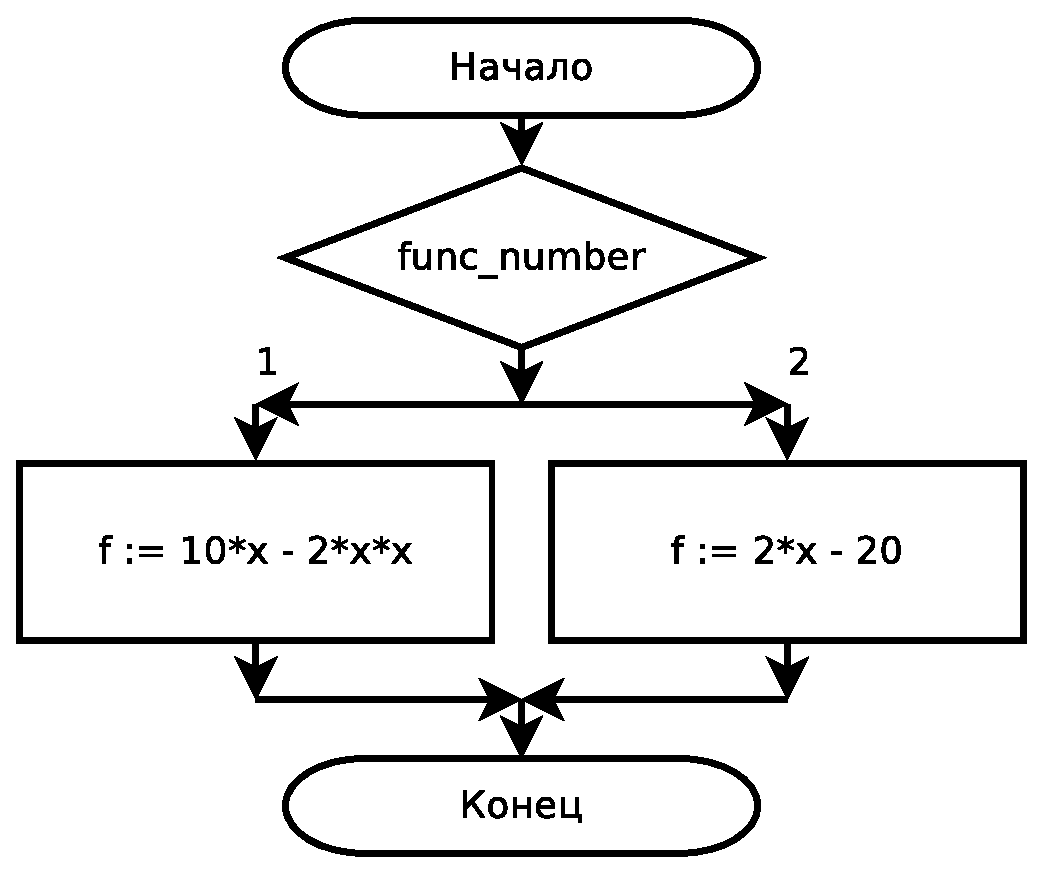
\includegraphics[scale=0.5]{schemes/f}

\subsection{Функция <<exact\_reached>>}
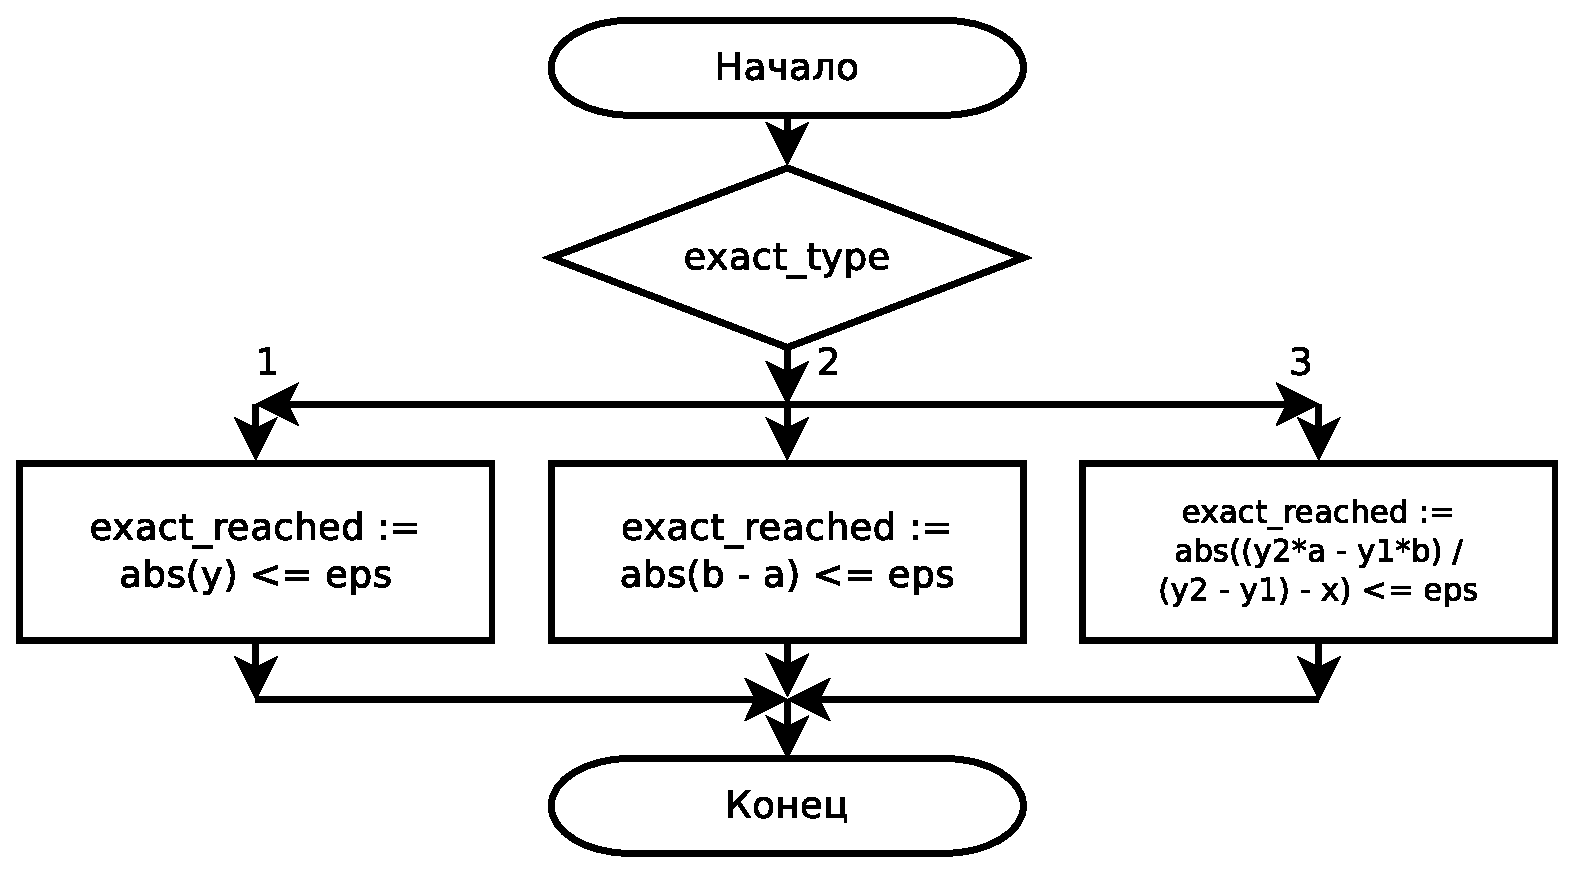
\includegraphics[scale=0.5]{schemes/exact_reached}

\subsection{Процедура <<calculate\_root>>}
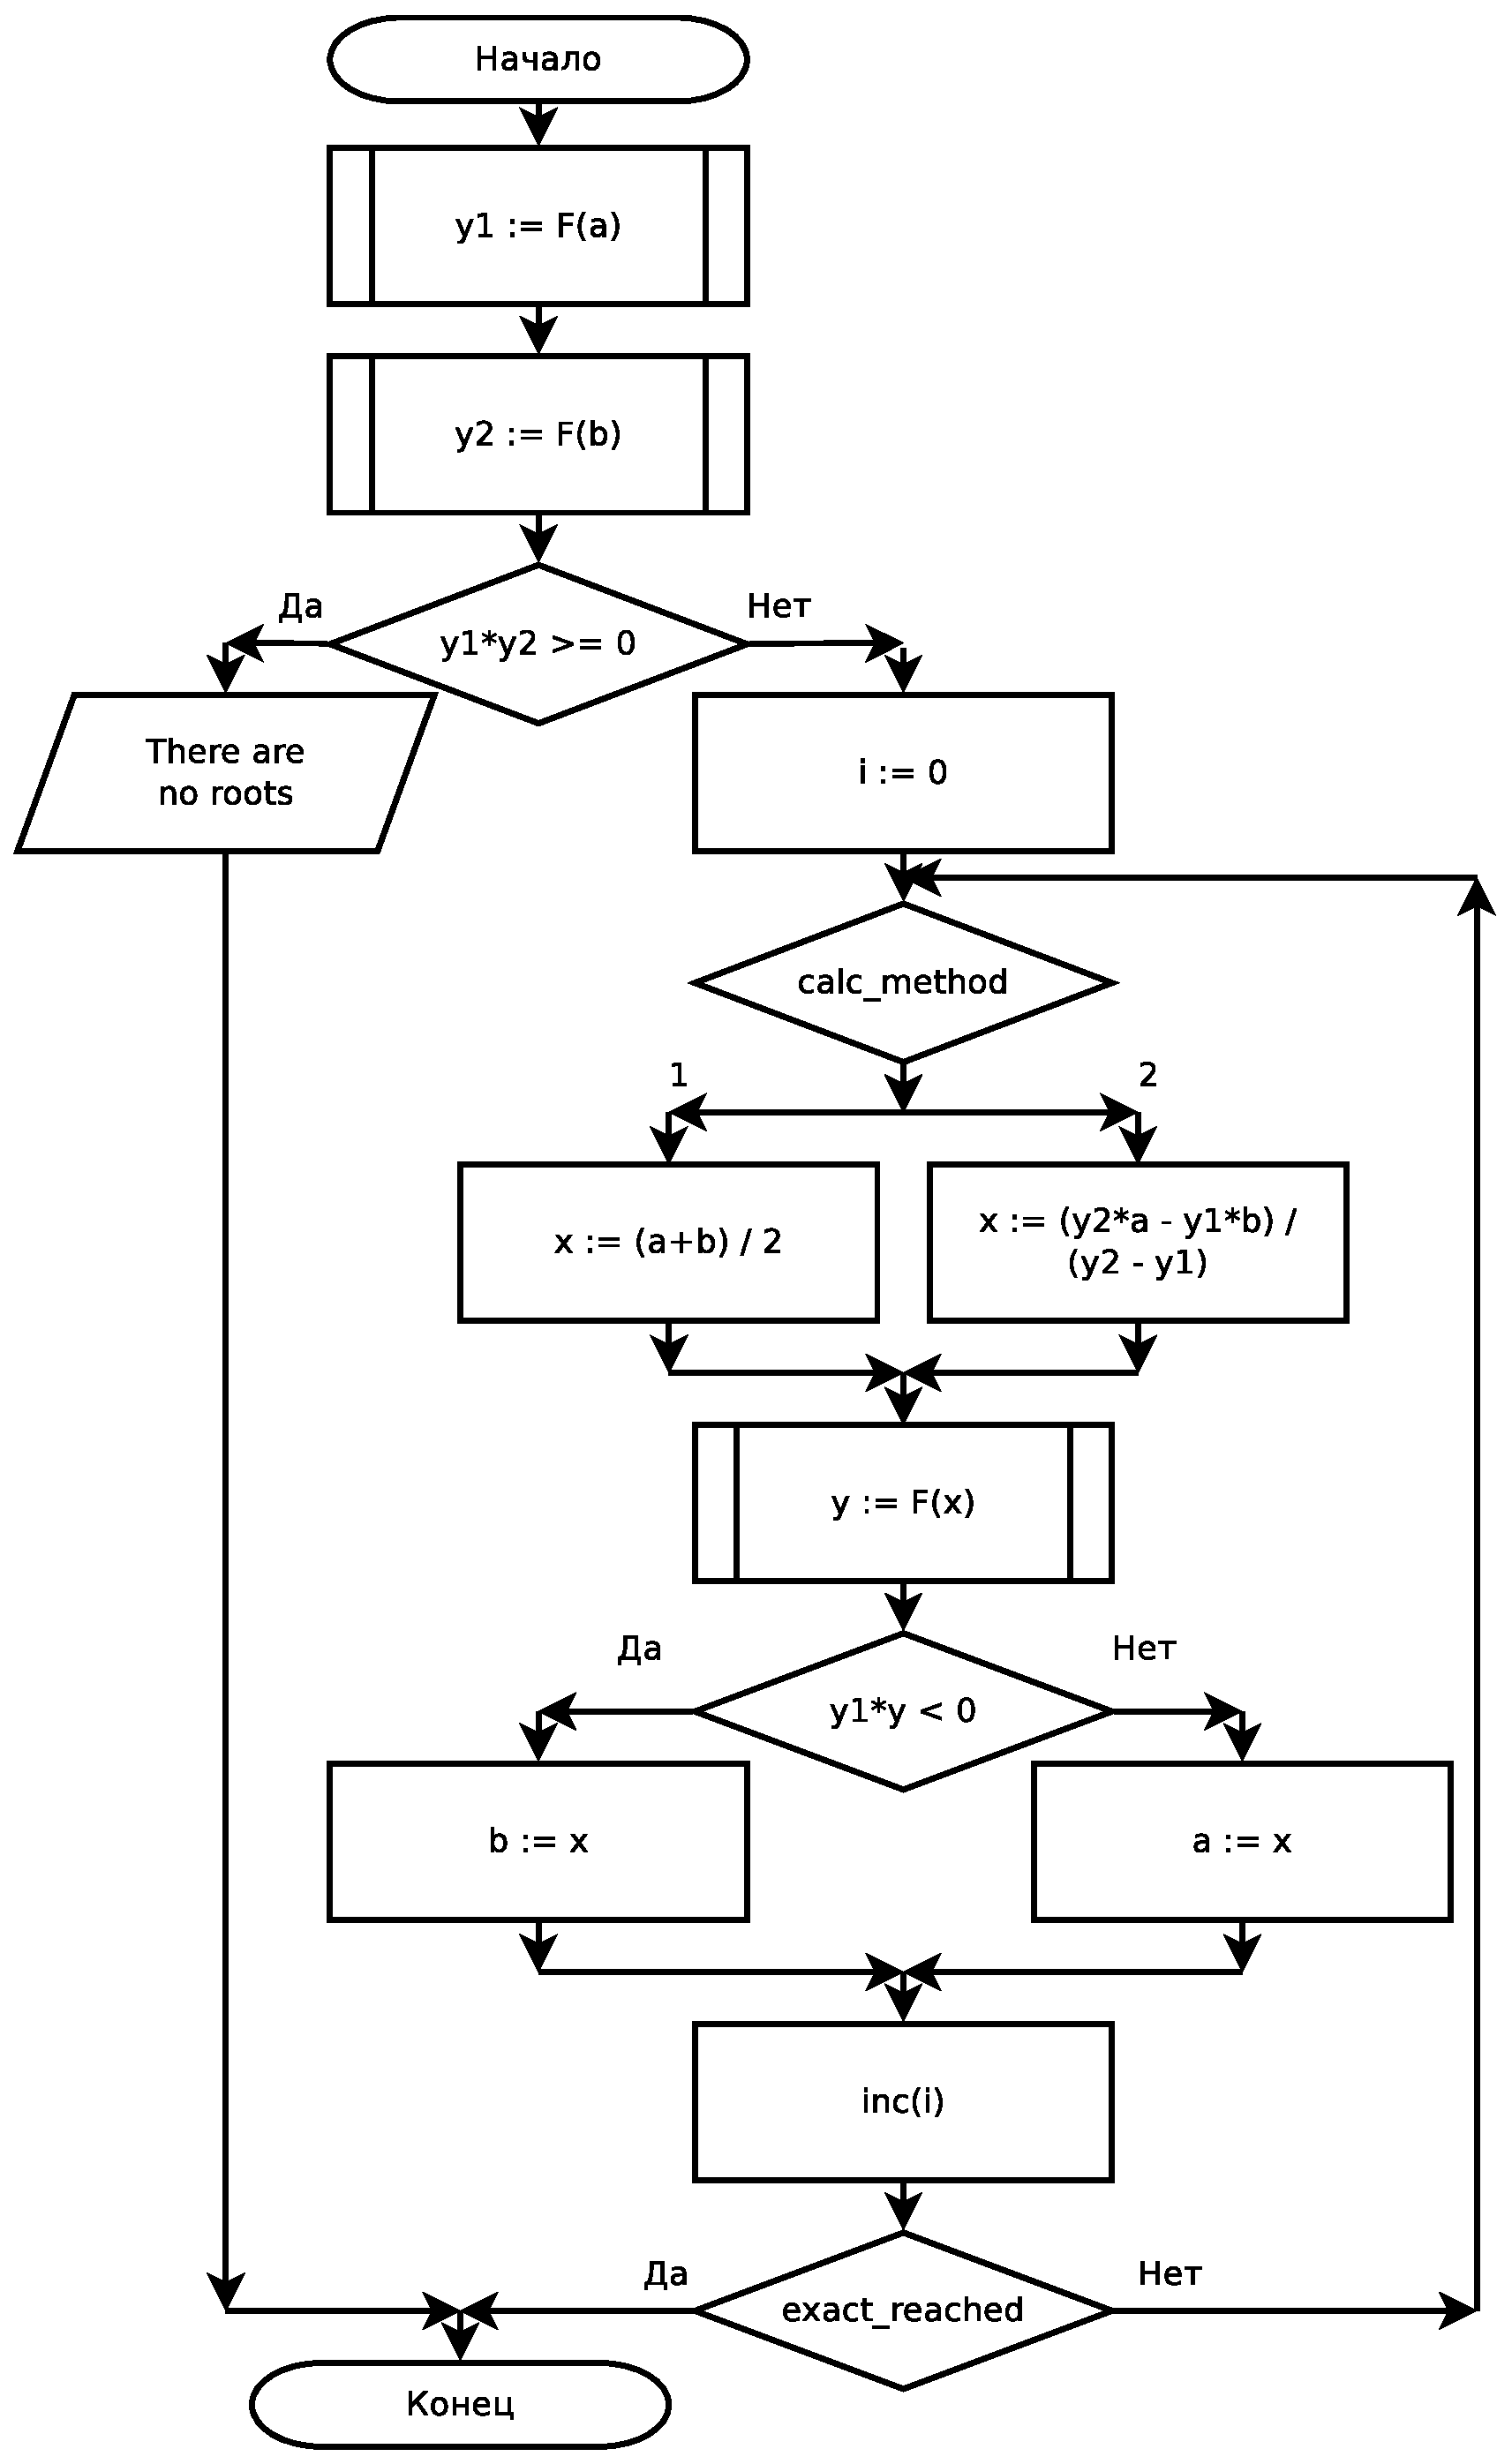
\includegraphics[scale=0.5]{schemes/calculate_root}

\subsection{Процедура <<print\_result>>}
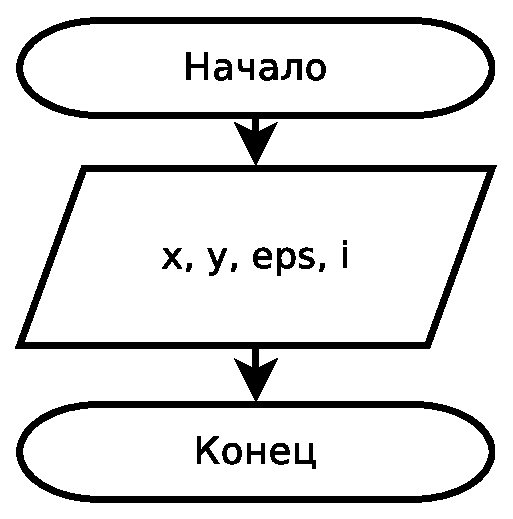
\includegraphics[scale=0.5]{schemes/print_result}

\section{Программа}
\verbatiminput{../1.pas}

\section{Шаблон ввода исходных данных}
\begin{verbatim}
1
100
0.01
1
1
1
\end{verbatim}

\section{Шаблон вывода результата}
\begin{verbatim}
x = 5.000122070312500, y = -0.001220732927322, eps = 0.010000000000000,
i = 13

\end{verbatim}

\section{Вывод}
После экспериментов с входными данными было выяснено следующее:
{
\newcounter{N}
\begin{list}{\arabic{N}.}{\usecounter{N}}
\item Наилучшую сходимость даёт метод хорд, но только если функция линейная
\item Проверять точность для метода хорд при поиске корня линейного уравнения
лучше всего по формуле $F(x)\le\varepsilon$, а при поиске корня квадратичного ---
через $y$ выраженный из уравнения прямой
\item Сходимость метода половинного деления примерно одинаковая на обеих
функциях и всех способах проверки точности, за исключением проверки точности
через $y$ выраженный из уравнения прямой --- этот способ совершенно неприменим
для метода половинного деления, т.~к. настоящий $y$, полученный с помощью
вычисления функции $F(x)$ сильно отличается от этого $y$ (однако количество
итераций при этом меньше по сравнению с остальными способами проверки точности)
\end{list}
}

\end{document}
